\setchapterimage[6.5cm]{seaside}
\setchapterpreamble[u]{\margintoc}
\chapter[Comandos y Ambientes]{Comandos y Ambientes\footnotemark[0]}
\labch{comenv}

\footnotetext{Los creditos para la portada del capitulo son de:
	Bushra Feroz --- Own work, CC~BY-SA~4.0, 
    \url{https://commons.wikimedia.org/w/index.php?curid=68724647}}

Esta es una plantilla de la clase Kaobook creada por Federico Marotta, cuya versión original en inglés puede encontrarse en su GitHub: \url{https://github.com/fmarotta/kaobook}, donde también se encuentra toda la documentacion y ejemplos. Esta plantilla esta modificada para que los distintos elementos de la clase se muestren en español. Esto incluye: las leyendas de las figuras y tablas, así como sus referencias en los textos; títulos de las secciones del frontmatter y el backmatter, como la tabla de contenidos, las referencias, el glosario, etc; asi como ambientes propios de de la clase, como teoremas, corolarios, definiciones, etc.

Adicionalmente, esta versión esta reordenada de tal forma que no sea necesario involucrarse con los archivos de configuración importantes a la hora de editar la plantilla. Basicamente cuenta con las siguientes carpetas y archivos:
\begin{itemize}
    \item \textbf{frontmatter:} el contenido previo al texto principal como:
    \begin{itemize}
        \item \textbf{cover.tex} La portada del libro, con el título y los autores.
        \item \textbf{copyright.tex} La página de derechos de autor.
        \item \textbf{dedication.tex} Una breve dedicación.
        \item \textbf{preface.tex} Prefacio del libro.
    \end{itemize} 
    \item \textbf{mainmatter:} el contenido principal del documento, el cual esta dividido en:
    \begin{itemize}
        \item \textbf{chapters:} capítulos.
        \begin{itemize}
            \item \textbf{comenv.tex} Comandos y Ambientes, las líneas que estas leyendo. 
        \end{itemize}
        \item \textbf{appendices:} apéndices.
        \begin{itemize}
            \item \textbf{appendix.tex} Apéndices de ejemplos, con listas y familias de fuentes.
        \end{itemize}
        \item \textbf{structure.tex} Aquí se construye la estructura de las partes, capítulos y apéndices del libro. 
    \end{itemize}
    \item \textbf{backmatter:} el contenido de la parte final del libro, que incluye:
    \begin{itemize}
        \item \textbf{references.bib} Las referencias bibliográficas.
        \item \textbf{nomenclature.tex} La nomeclatura o notación utilizada en el libro.
        \item \textbf{glossary.tex} El glosario del libro con las siglas, abreviaciones y términos especiales. 
    \end{itemize}
    \item \textbf{images:} aquí van las imagenes del libro.
    \begin{itemize}
        \item \textbf{monalisa.jpg} La mona lisa.
        \item \textbf{seaside.jpeg} Una playa.  
    \end{itemize}
    \item \textbf{styles:} los archivos que contienen la información pertinente a los paquetes utilizados, ambientes creados, definiciones, configuraciones, estilos. No deberías modificar los archivos de esta carpeta.
    \item \textbf{kaobook.cls} El archivo que contiene la información pertinente a la clase kaobook, no deberías modificarlo.
    \item \textbf{main.tex} El archivo principal de la plantilla, todo se compila desde aquí. No es necesario modificarlo a menos que quieras editar cosas referidas al backmatter.
    \item \textbf{README.md} Archivo Leeme
\end{itemize}

Reiterando, la idea es que no es necesario que modifiques los archivos \emph{kaobook.cls}, \emph{main.tex} y todos aquellos que están en la carpeta \emph{styles} para utilizar esta plantilla. Toda la edición del libro se hace en las carpetas \emph{frontmatter}, \emph{mainmatter} y \emph{backmatter}. Las figuras se guardan en la carpeta \emph{images}. 

Una buena advertencia, esta plantilla no es para usuarios novatos en \LaTeX. De aquí viene la intención de dejar ordenados los archivos de la manera descrita, es decir, para alejarte de los elementos vitales de la clase. De esta forma te podes concentrar simplemente en la edición dentro de las carpetas \emph{frontmatter}, \emph{mainmatter}, \emph{backmatter} e \emph{images} sin correr peligro de desconfigurar o dejar fuera de funcionamiento los comandos y ambientes definidos en el resto de los archivos.

Es mas que recomendable leer la documentación que se encuentra en el GitHub del autor original. Aquí solo se muestran las cosas que fueron traducidas al español, el potencial de esta clase es mucho mejor explicitado allí. En lo personal, me gusta mucho todas las herramientas que brinda y aspecto en si. No me gustan los textos que tienen lineas de texto que abarcan toda la hoja, pero tampoco me gusta los enormes margenes que se suelen dejar a ambos costados para evitar esto. Los textos con doble columna, o varias de ellas, pueden resultar muy cansadores de leer. La clase kaobook brinda un ambiente de una única columna, no centrada, de un tamaño razonable y utiliza inteligentemente el margen sobrante para colocar figuras, tablas, ecuaciones, notas al margen, código de programación, cajas, etc. Además brinda herramientas útiles para escribir textos de ciencia e ingenería, que incluyen gran cantidad de imágenes, tablas, ecuaciones, teoremas, definiciones, etc.; donde tener todo correctamente referenciado es la diferencia entre un buen texto y uno tedioso de leer.

En el resto de las secciones se muestran los distintos comandos y ambientes traducidos al español. Los ejemplos se toman de la documentacion original en inglés.
    
\section{Figuras y Tablas}
\labsec{figytab}
En la clase kaobook se pueden poner tres tipos de tablas y figuras: las <<\emph{normales}>>, las que van en los <<\emph{márgenes}>>, y las <<\emph{anchas}>> que ocupan todo el ancho de la hoja.

\subsection{Figuras y Tablas Normales}
\index{Figura} \index{Tabla}

Las figuras y tablas normales usan los ambientes más comunes de \LaTeX para insertar estos objetos: \Environment{figure} y \Environment{table}. Por ejemplo, aquí hay una imagen de la Mona Lisa \reffig{normalmonalisa}. Puede verse que la leyenda se muestra comodamente en el amplio margen a su costado y tanto este como la referencia en el texto se muestran en español.

\begin{figure}[hb]
	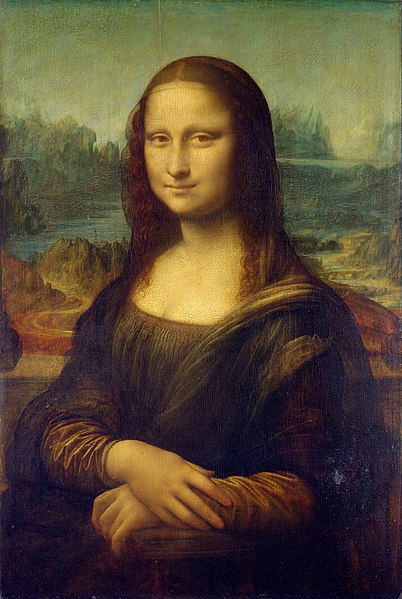
\includegraphics[width=0.45\textwidth]{monalisa}
	\caption[La Mona Lisa]{La Mona Lisa. \blindtext}
	\labfig{normalmonalisa}
\end{figure}

Las tablas pueden ser insertadas igual de fácil que las figuras, como se ejemplifica en el siguiente código:

\begin{lstlisting}[caption={Leyenda de un Código.}]
\begin{table}
\begin{tabular}{ c c c c }
	\toprule
	col1 & col2 & col3 & col 4 \\
	\midrule
	\multirow{3}{4em}{Multiple row} & cell2 & cell3 & cell4\\ &
	cell5 & cell6 & cell7 \\ &
	cell8 & cell9 & cell10 \\
	\multirow{3}{4em}{Multiple row} & cell2 & cell3 & cell4 \\ &
	cell5 & cell6 & cell7 \\ &
	cell8 & cell9 & cell10 \\
	\bottomrule
\end{tabular}
\end{table}
\end{lstlisting}

el cual resulta en la inútil \vreftab{useless}.

\begin{table}[h]
\caption[Una Tabla Inútil]{Una Tabla Inútil.}
\labtab{useless}
\begin{tabular}{ c c c c }
	\toprule
	col1 & col2 & col3 & col 4 \\
	\midrule
	\multirow{3}{4em}{Multiple row} & cell2 & cell3 & cell4\\ &
	cell5 & cell6 & cell7 \\ &
	cell8 & cell9 & cell10 \\
	\multirow{3}{4em}{Multiple row} & cell2 & cell3 & cell4 \\ &
	cell5 & cell6 & cell7 \\ &
	cell8 & cell9 & cell10 \\
	\bottomrule
\end{tabular}
\end{table}

\subsection{Figuras y Tablas al Margen}
Las figuras al margen se insertan utilizando el ambiente \Environment{marginfigure}. En este caso toda la imagen esta confinada en el margen y la leyenda se muestra debajo de ella. La \reffig{marginmonalisa} se obtiene con algo como esto:

\begin{lstlisting}[caption={Otra leyenda.}]
\begin{marginfigure}
    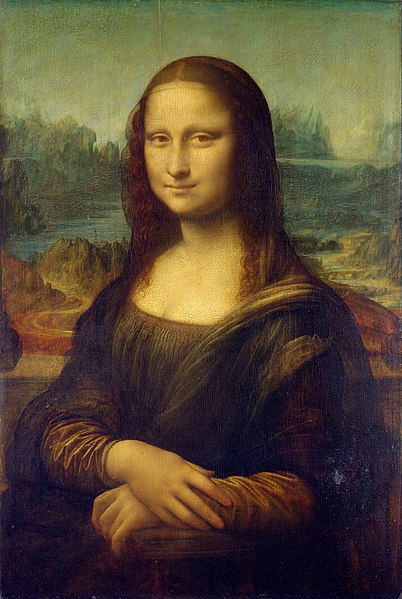
\includegraphics{monalisa}
    \caption[The Mona Lisa]{The Mona Lisa.}
    \labfig{marginmonalisa}
\end{marginfigure}
\end{lstlisting}

\begin{marginfigure}[0cm]
	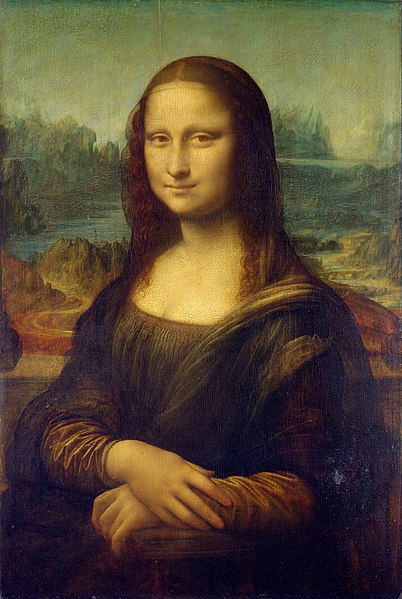
\includegraphics{monalisa}
	\caption[La Mona Lisa, una vez mas.]{La Mona Lisa, una vez mas.\\ 
	\url{https://commons.wikimedia.org/wiki/File:Mona_Lisa,_by_Leonardo_da_Vinci,_from_C2RMF_retouched.jpg}}
	\labfig{marginmonalisa}
\end{marginfigure}

También hay un ambiente \Environment{margintable}, del cual la \reftab{anotheruseless} es un ejemplo. Nota como podés colocar la leyenda encima de la tabla simplemente colocando el comando \Command{caption} antes de comenzar el ambiente \Environment{tabular}. Usualmente, las leyendas de las figuras estan debajo, mientras que las leyendas de las tablas estan por encima de ellas. Esta regla también se aplica a las figuras y tablas <<\emph{normales}>>: la leyenda siempre esta al costado, pero para las figuras estan alineadas a con el borde inferior de la figura, mientras que para las tablas lo estan para el borde superior.

\begin{margintable}
    \caption[Otra tabla inútil]{Otra tabla inútil.}
    \labtab{anotheruseless}
    \raggedright
    \begin{tabular}{ c c c c }
        \hline
        col1 & col2 & col3 \\
        \hline
        \multirow{3}{4em}{Multiple row} & cell2 & cell3 \\ & cell5 & cell6 
        \\ & cell8 & cell9 \\ \hline
    \end{tabular}
\end{margintable}

Las figuras y tablas al margen puede ser reposicionadas colocando un offset, como se muestra en este código:
    
\begin{lstlisting}
\begin{marginfigure}[offset]
    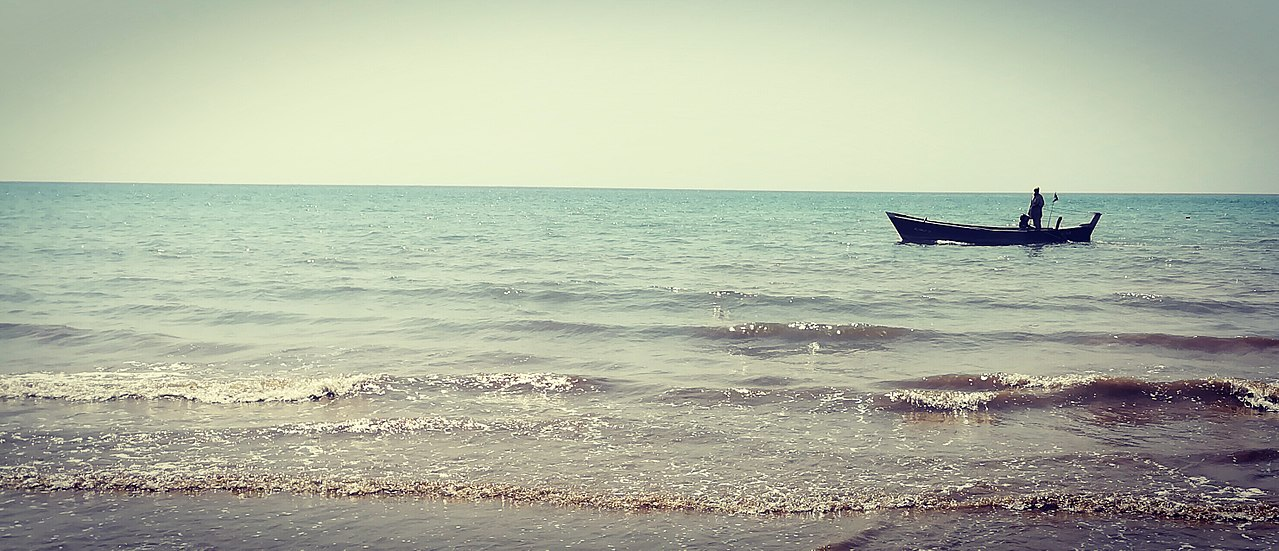
\includegraphics{seaside}
\end{marginfigure}
\end{lstlisting}

\subsection{Figuras y Tablas Anchas}

\begin{figure*}[h!]
	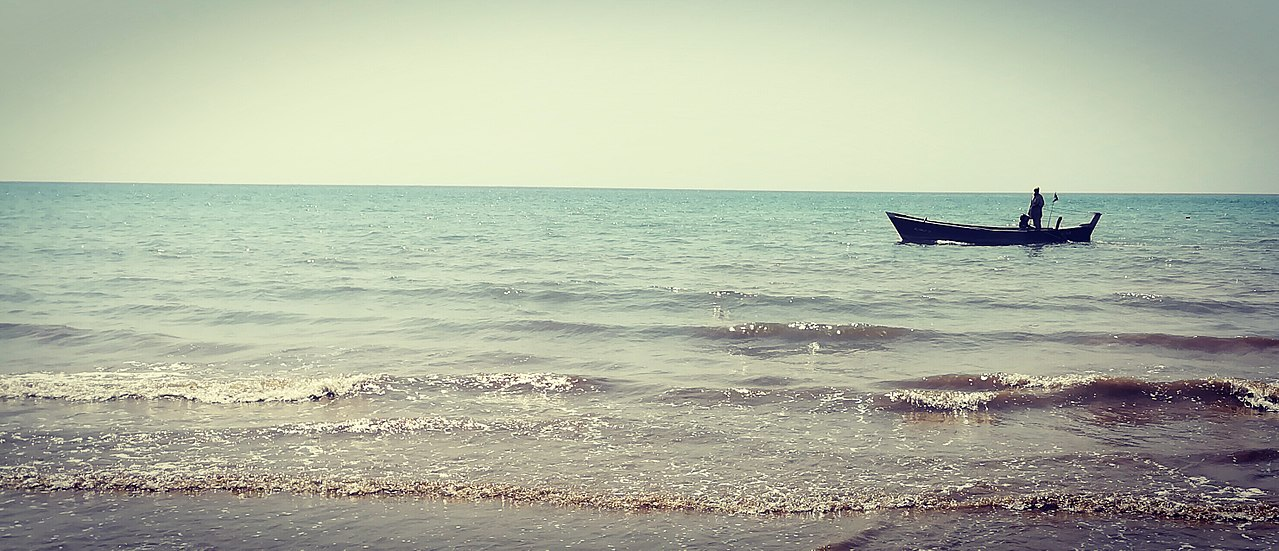
\includegraphics{seaside}
    \caption[Una playa ancha]{Una playa ancha, y una leyenda ancha. Creditos: Por Bushra Feroz --- Trabajo propio, CC BY-SA 4.0, \url{https://commons.wikimedia.org/w/index.php?curid=68724647}}
    \labfig{widefigure}
\end{figure*}

Con los ambientes \Environment{figure*} y \Environment{table*} podes insertar figuras que ocupen todo el ancho de la página, como la mostrada en la \reffig{widefigure}. La leyenda estara posicionada por debajo o por encima, acorde al gusto.

\section{Matemática e Hiperreferencias}
\labpage{unapagina}
\subsection{Teoremas}
Acá ilustro como se ven los ambientes \Environment{definition}, \Environment{theorems}, \Environment{proposition}, \Environment{lemma}, \Environment{corollary}, \Environment{proof}, \Environment{example}, \Environment{remark}, en español.

\index{Definición}
\begin{definition}
    \labdef{unadefinicion}
    Let $(X, d)$ be a metric space. A subset $U \subset X$ is an open set if, for any $x \in U$ there exists $r > 0$ such that $B(x, r) \subset U$. We call the topology associated to d the set $\tau\textsubscript{d}$ of all the open subsets of $(X, d).$
\end{definition}

La \refdef{unadefinicion} es muy importante. No es una broma, pero inserté esta frase solo para mostrar como referenciar las definiciones. Esta declaración es repetida una y otra vez en distintos ambientes.

\index{Teorema}
\begin{theorem}
    \labthm{unteorema}
    A finite intersection of open sets of (X, d) is an open set of (X, d), i.e $\tau\textsubscript{d}$ is closed under finite intersections. Any union of open sets of (X, d) is an open set of (X, d).
\end{theorem}

\begin{proposition}
    \labprop{unaproposicion}
    A finite intersection of open sets of (X, d) is an open set of (X, d), i.e $\tau\textsubscript{d}$ is closed under finite intersections. Any union of open sets of (X, d) is an open set of (X, d).\marginnote{Podés incluso insertar notas al pie dentro de los ambientes matemáticos; se mostrarán en la parte inferior de la caja.}
\end{proposition}

\begin{lemma}
    \lablemma{unlema}
    A finite intersection\footnote{Soy una nota al pie} of open sets of (X, d) is an open set of (X, d), i.e $\tau\textsubscript{d}$ is closed under finite intersections. Any union of open sets of (X, d) is an open set of (X, d).
\end{lemma}

Podés ignorar el contenido de los teoremas\ldots asumo que si estas interesado en tener teoremas en tu libro, ya sabés algo acerca de la manera clásica de colocarlos. Estos ejemplos deberían mostrar las cosas que podés hacer con esta clase.

\begin{corollary}[Finite Intersection, Countable Union]
    \labcoro{uncorolario}
    A finite intersection of open sets of (X, d) is an open set of (X, d), i.e $\tau\textsubscript{d}$ is closed under finite intersections. Any union of open sets of (X, d) is an open set of (X, d).
\end{corollary}

\begin{proof}
    The proof is left to the reader as a trivial exercise. Hint: \blindtext
\end{proof}

\begin{definition}
Let $(X, d)$ be a metric space. A subset $U \subset X$ is an open set if, for any $x \in U$ there exists $r > 0$ such that $B(x, r) \subset U$. We call the topology associated to d the set $\tau\textsubscript{d}$ of all the open subsets of $(X, d).$\marginnote{
	Aqui hay otra ecuación cualquiera, solo porque se puede:
	\begin{equation*}
  x = a_0 + \cfrac{1}{a_1
          + \cfrac{1}{a_2
          + \cfrac{1}{a_3 + \cfrac{1}{a_4} } } }
	\end{equation*}
}
\end{definition}

\begin{example}
    \labexample{unejemplo}
    Let $(X, d)$ be a metric space. A subset $U \subset X$ is an open set if, for any $x \in U$ there exists $r > 0$ such that $B(x, r) \subset U$. We call the topology associated to d the set $\tau\textsubscript{d}$ of all the open subsets of $(X, d).$
\end{example}

\begin{remark}
    \labremark{unaobservacion}
    Let $(X, d)$ be a metric space. A subset $U \subset X$ is an open set if, for any $x \in U$ there exists $r > 0$ such that $B(x, r) \subset U$. We call the topology associated to d the set $\tau\textsubscript{d}$ of all the open subsets of $(X, d).$
\end{remark}

Como podrías haber notado, las definiciones, ejemplos y las observaciones tienen contadores independientes; los teoremas, proposiciones, lemas y corolarios comparten el mismo contador.

\begin{remark}
    Here is how an integral looks like inline: $\int_{a}^{b} x^2 dx$, and here is the same integral displayed in its own paragraph: \[\int_{a}^{b} x^2 dx\]
\end{remark}

\subsection{Citas y Referencias}
\index{Referencias}
Algunos ejemplos de como referenciar distintas cosas: \refdef{unadefinicion}, \refthm{unteorema}, \refprop{unaproposicion}, \reflemma{unlema}, \refcoro{uncorolario}, \refremark{unaobservacion},\refexample{unejemplo}. 

También se pueden citar distintas partes de la estructura del libro.
\begin{itemize}
    \item Partes:
    \begin{itemize}
        \item \arefpart{contprinp}
        \item \avrefpart{contprinp}
    \end{itemize}
    \item Capítulos:
    \begin{itemize}
        \item \refchshort{comenv}
        \item \refch{comenv}
        \item \vrefch{comenv}
        \item \nrefch{comenv}
        \item \frefch{comenv}
    \end{itemize}
    \item Secciones:
    \begin{itemize}
        \item \refsecshort{figytab}
        \item \refsec{figytab}
        \item \vrefsec{figytab}
        \item \nrefsec{figytab}
        \item \frefsec{figytab}
    \end{itemize}
    \item Páginas:
    \begin{itemize}
        \item \refpage{unapagina}
        \item \vrefpage{unapagina}
    \end{itemize}
\end{itemize}

Esta es una ecuación:
\begin{equation}
    x_{1,2}=\frac{-b\pm\sqrt{b^2-4ac}}{2a}
    \labeq{unaecuacion}
\end{equation}
y así es como luce referenciada: \refeq{unaecuacion}.

En este parrafo ilustramos como se ven distintos elementos del backmatter, como las referencias bibliograficas: \sidecite{Ardlie2015,Visscher2008,Gusev2018}; elementos del glosario: \acrfull{fpsLabel}, \gls{computer}, \acrshort{fpsLabel}. Y usando el comando \Command{index}, podemos indicarle al indice donde esta una palabra de interés. \index{Indice}.




